\subsection{Kortslutningssikring}
\label{effekt_kortslutningssikring}
Kortslutningssikringen tilføjes ved at indføre kredsløbet, vist på figur \ref{fig:dia-kortslut}, som vist på figur \ref{fig:dia-kortslut1}. 

\begin{figure}[h]
\centering
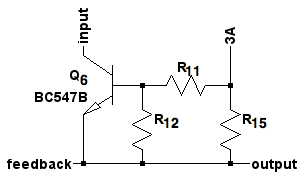
\includegraphics[scale=1]{teknisk/effektforstaerker/diagram-kortslut.png}
\caption{Overordnet diagram over kortslutningssikringens aktiveringssituation}
\label{fig:dia-kortslut}
\end{figure}

Strømmen på 3 A, anført på figur \ref{fig:dia-kortslut}, er den strøm, hvor kortslutningssikringen skal aktivere, hvilket blev bestemt i afsnit \ref{valg_kortslutningssikring}. At kortslutningssikringen skal aktivere betyder her, at transistoren Q1 skal åbnes. 

\begin{figure}[h]
\centering
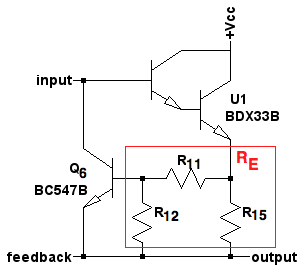
\includegraphics[scale=1]{teknisk/effektforstaerker/diagram-kortslut1.png}
\caption{Overordnet diagram over kortslutningssikring forbundet darlingtontransistor}
\label{fig:dia-kortslut1}
\end{figure}

Modstandene $R_1$, $R_2$ og $R_3$ skal, som vist på figur \ref{fig:dia-kortslut1}, repræsentere samme modstandsværdi som $R_E$ beregnet i afsnit \ref{effekt_stroemforstaerker}, da den stadig skal sikre termisk stabilitet. 

\subsubsection*{Simulering}